\documentclass[tikz,border=2mm]{standalone}
\usetikzlibrary{trees,positioning}

\begin{document}

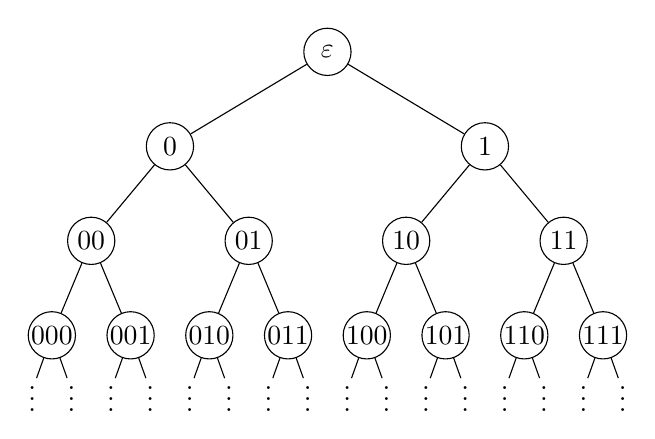
\begin{tikzpicture}[
	level distance=1.2cm,
	level 1/.style={sibling distance=4cm},
	level 2/.style={sibling distance=2cm},
	level 3/.style={sibling distance=1cm},
	level 4/.style={
		sibling distance=0.5cm,
		every node/.style={
			minimum size=0mm,
			inner sep=0pt,
			yshift=5mm
		}
	},
	every node/.style={circle,draw,minimum size=6mm,inner sep=0pt}
]

\node {$\varepsilon$}
	child { node {0} 
		child { node {00} 
			child { node {000} 
				child { node {$\vdots$} }
				child { node {$\vdots$} }
			}
			child { node {001} 
				child { node {$\vdots$} }
				child { node {$\vdots$} }
			}
		}
		child { node {01} 
			child { node {010} 
				child { node {$\vdots$} }
				child { node {$\vdots$} }
			}
			child { node {011} 
				child { node {$\vdots$} }
				child { node {$\vdots$} }
			}
		}
	}
	child { node {1} 
		child { node {10} 
			child { node {100} 
				child { node {$\vdots$} }
				child { node {$\vdots$} }
			}
			child { node {101} 
				child { node {$\vdots$} }
				child { node {$\vdots$} }
			}
		}
		child { node {11} 
			child { node {110} 
				child { node {$\vdots$} }
				child { node {$\vdots$} }
			}
			child { node {111} 
				child { node {$\vdots$} }
				child { node {$\vdots$} }
			}
		}
	};

\end{tikzpicture}

\end{document}
